\chapter{PLONK Rounds}

Now that we finally have all of the components needed let's construct the protocol. The $\plonk$ protocol has a one-time trusted setup algorithm that generates the common preprocessed input. Part of this setup is to generate the \textit{structured reference string} for polynomial commitments. The prover has a routine proving algorithm that is split into 5 rounds in the original paper, this is the approach we will take as well. Finally, there is an algorithm for the verifier, that is very much implicit. There will be a provided diagram to show how the protocol works. Below is the legend for these diagrams.


\begin{figure}[H]
    \centering
    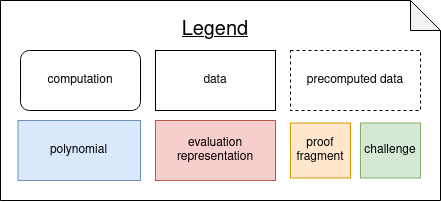
\includegraphics[width=0.5\linewidth]{round-figures/legend.drawio.png}
    \caption{Legend for the Plonk diagrams}
    
\end{figure}



\begin{figure}[ht]
    \centering
    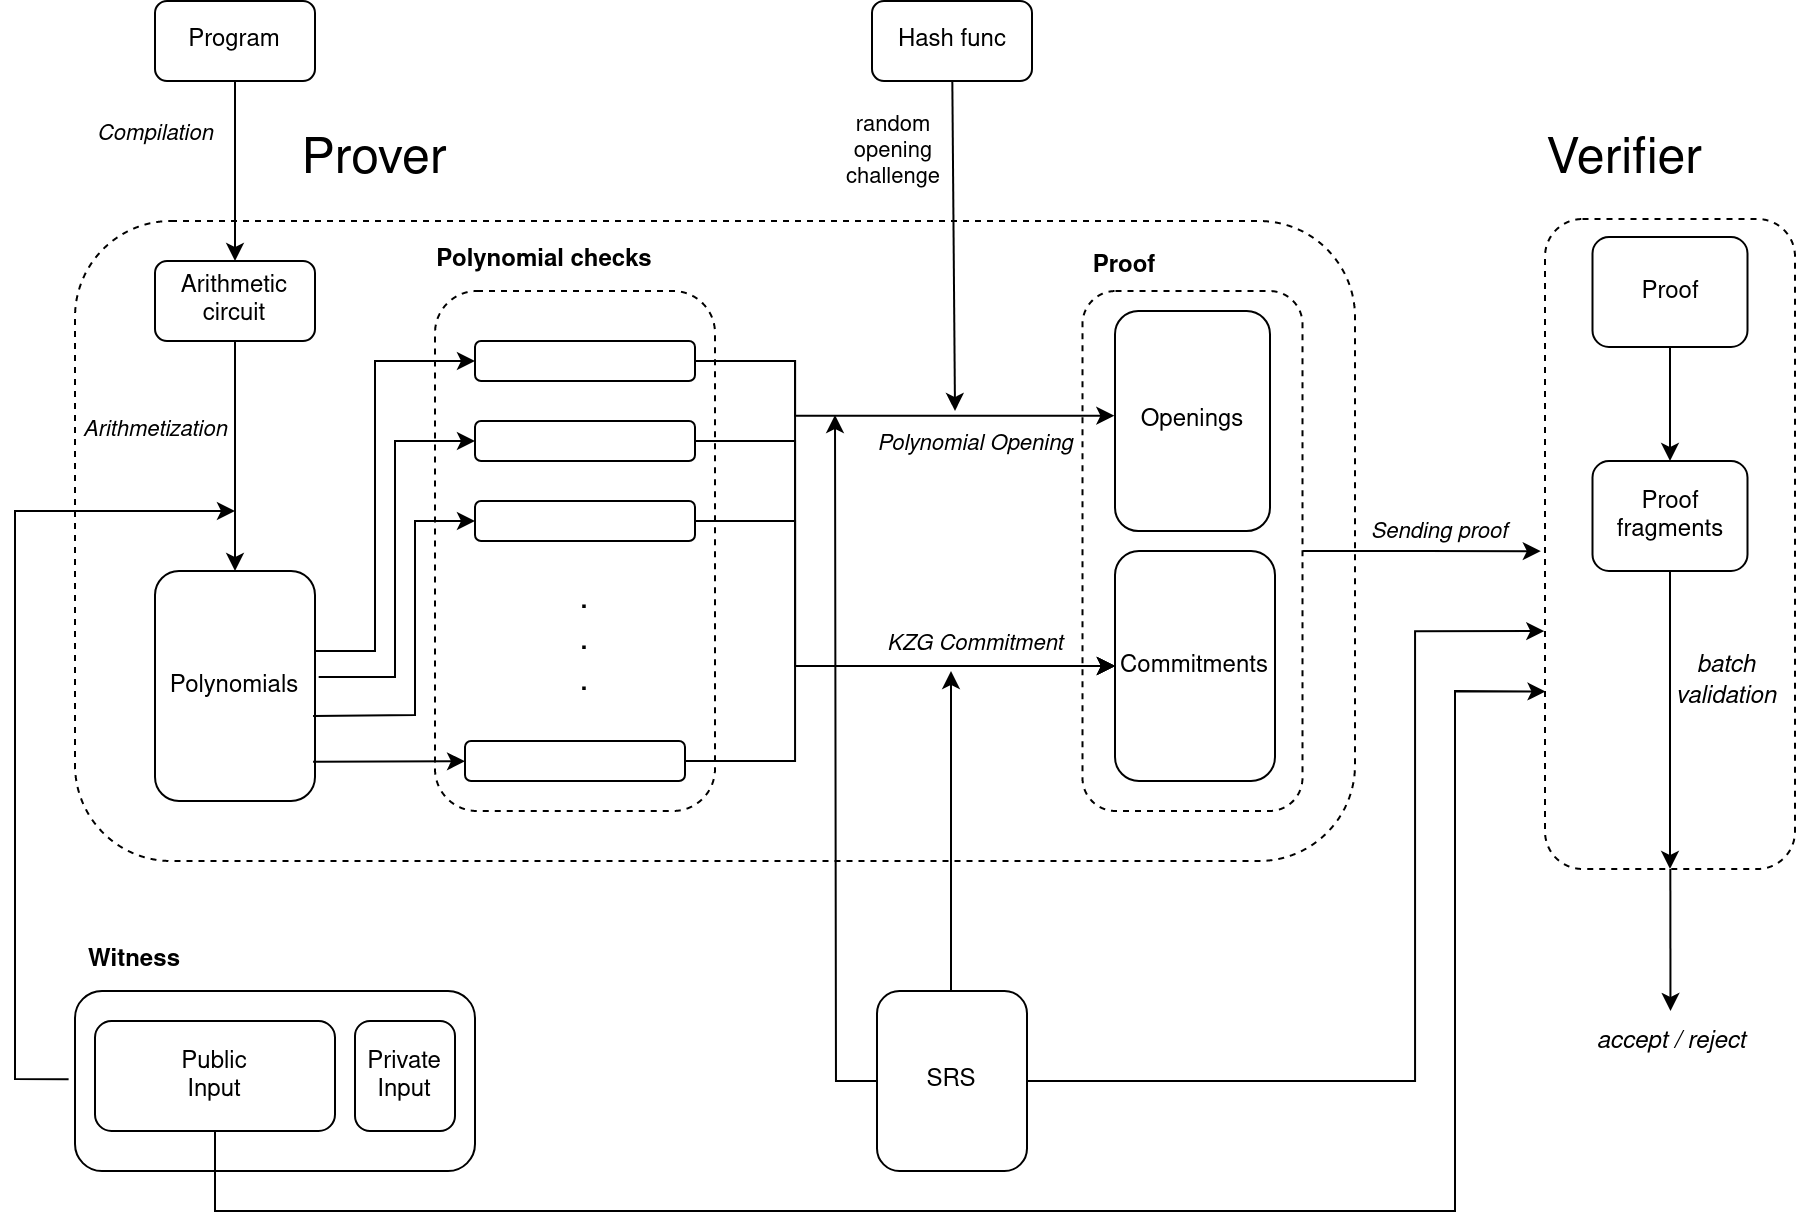
\includegraphics[width=1\linewidth]{round-figures/round1/plonk_better_overview.drawio.png}
\end{figure}

Throughout reading the protocol keep in mind that we will be aiming for following complexities:
\begin{itemize}
    \item proof size: $O(\log{d})$
    \item verifier time: $O(\log{d})$
    \item prover time: do not know need to find
\end{itemize}

% ==============================================================================
% ===SETUP======================================================================
% ==============================================================================
\section{Setup algorithm}
\label{chap:round0}
The setup algorithm describes the calculation of the common pre-processed input. It is not considered a routine protocol round. The only trusted part is the public key \textit{structured reference string} $SRS$ that is not tied to the structure of an arithmetic circuit but to the upper bound of the number of the circuit gates. This means that the circuit could be updated without the need to perform a trusted setup and $SRS$ can be reused. It is important to note that the $SRS$ cannot be generated by the prover because discovering the key $\tau$ would allow one to forge commitments and therefore give invalid evaluations.

\begin{figure}[H]
    \centering
    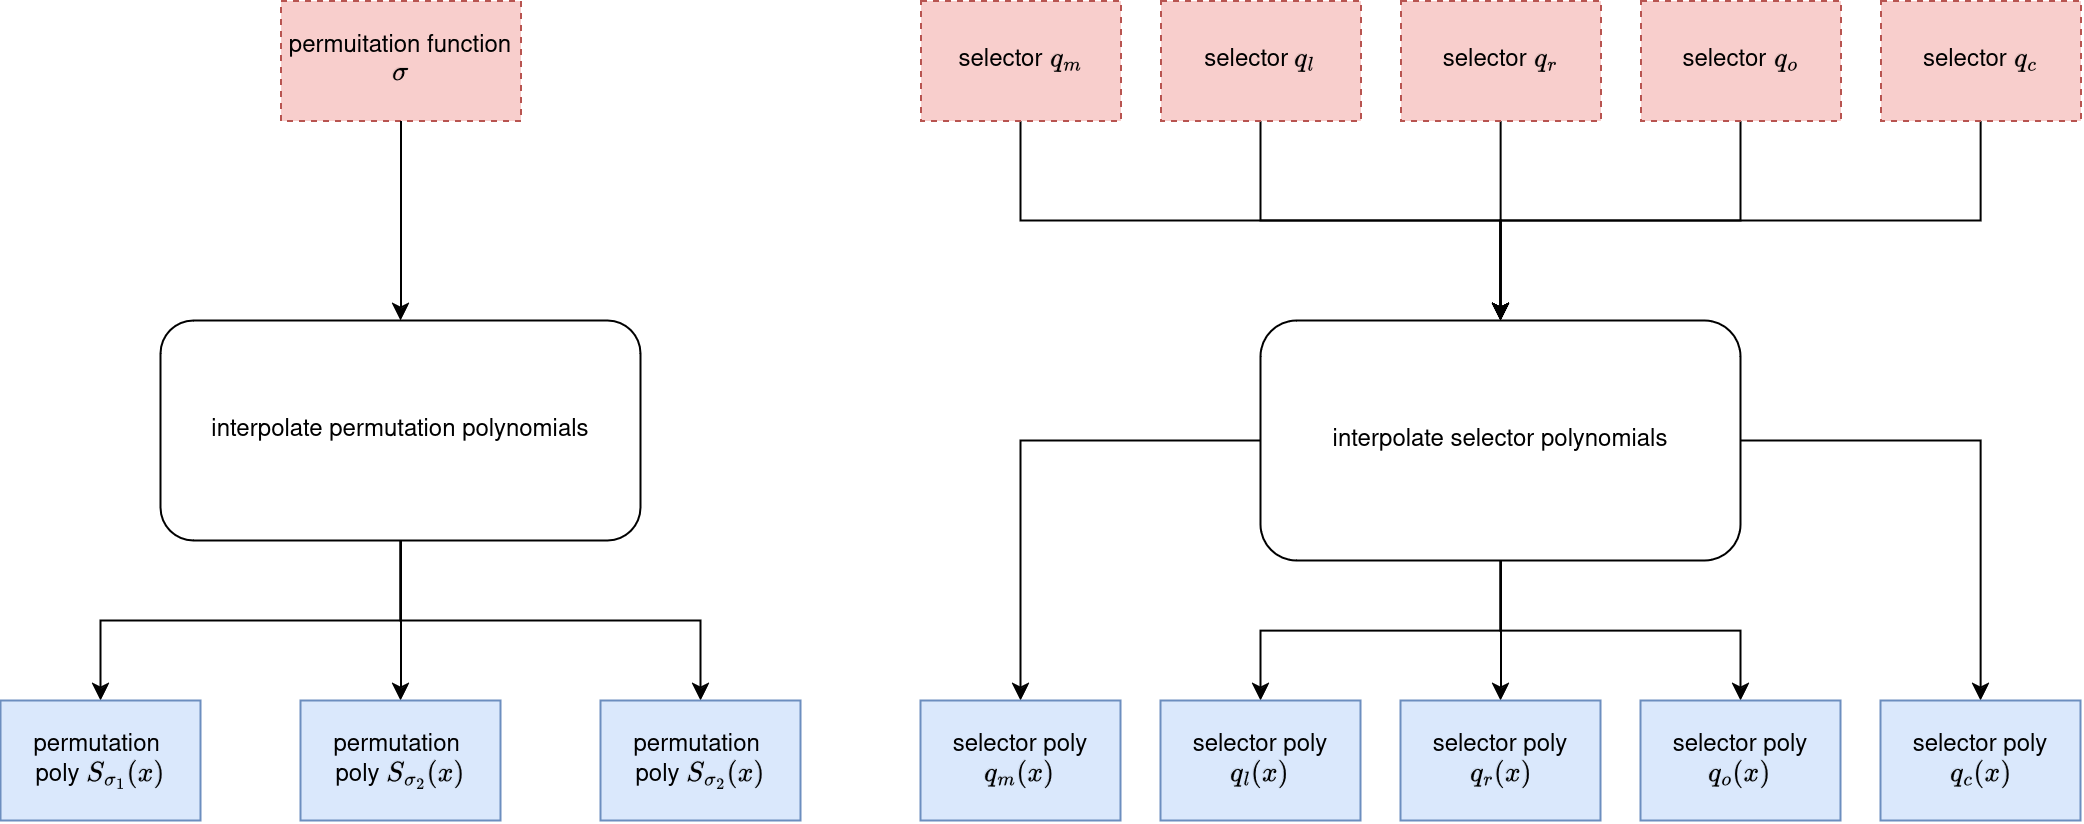
\includegraphics[width=1\linewidth]{round-figures/setup/round0.drawio.png}
    \caption{Setup algorithm}
    
\end{figure}


\subsection{Public Information }
All of the parties have information $(\field, \mathbb{G}_1, \mathbb{G}_2, \mathbb{G}_t, e, G_1, G_2, G_t, SRS)$ where $\field$ is a prime field, $(\mathbb{G}_1, \mathbb{G}_2, \mathbb{G}_t)$ are groups of points on elliptic curves and $e$ is efficiently computable group pairing $e: \mathbb{G}_1 \times \mathbb{G}_2 \rightarrow \mathbb{G}_t$. Lastly $G_1, G_2$ are group generators for which holds $e(G_1, G_2) = G_t$. All of the information above needs to be available to any party to perform arithmetic operations on elliptic curves. Moreover, there needs to be a KZG setup ceremony generating the \textit{structured reference string} SRS which is public.

Some input to the circuit might be public. This means we are able to split the witness $w$ into public $w_{pub} = (w_i)_{i\in [l]}$ and private $w_{priv} = (w_i)_{i = l+1}^{3n}$ where $l < n$ is the number of public inputs to the circuit. The public input is encoded as a polynomial:
$$PI(x) = \sum_{i \in [l]} - w_{pub_i} L_i(x)$$


\subsection{Preprocessed Input}
Below is summed up the common preprocessed input that is available to both parties. Each of the components will be described in detail in the following rounds.

\begin{itemize}
    \item number of gates: $n$
    \item $k_1, k_2 \in \field$ are needed to create cosets $k_1 H , k_2 H$ of group $H$ such that the union $H' = H \cup k_1 H \cup k_2H)$ contains $3n$ distinct elements. This will be explained in the round 2.
    \item $SRS$ for KZG: $([1]_1, [\tau]_1, [\tau^2]_1, ..., [\tau^{n+5}]_1, [1]_2, [\tau]_2)$ 
    \item permutation function: $\sigma^*: [3n] \rightarrow H'$ 
    \item selector polynomials: $q_m(x), q_l(x), q_r(x), q_o(x), q_c(x)$ interpolated from selector vectors explained in arithmetization
    \item permutation polynomials: $S_{\sigma_1}, S_{\sigma_2}, S_{\sigma_3}$ interpolated from $\sigma^*$ in detail in round 2
\end{itemize}


% ==============================================================================
% ===ROUND1=====================================================================
% ==============================================================================
\section{Round 1}
\label{chap:round1}

The proof generation starts by computing the wire polynomials and committing to them. In this chapter, we will also explain:

Round overview:
\begin{enumerate}
    \item Generate random blinding scalars $(b_1, ... b_9) \in \field$ just some numbers needed to introduce randomness 
    \item Compute wire polynomials $a, b, c$
    \item Compute and output commitments $[a]_1, [b]_1, [c]_1 \in \mathbb{G}_1$ 
\end{enumerate}

\begin{figure}[H]
    \label{fig:round1}
    \centering
    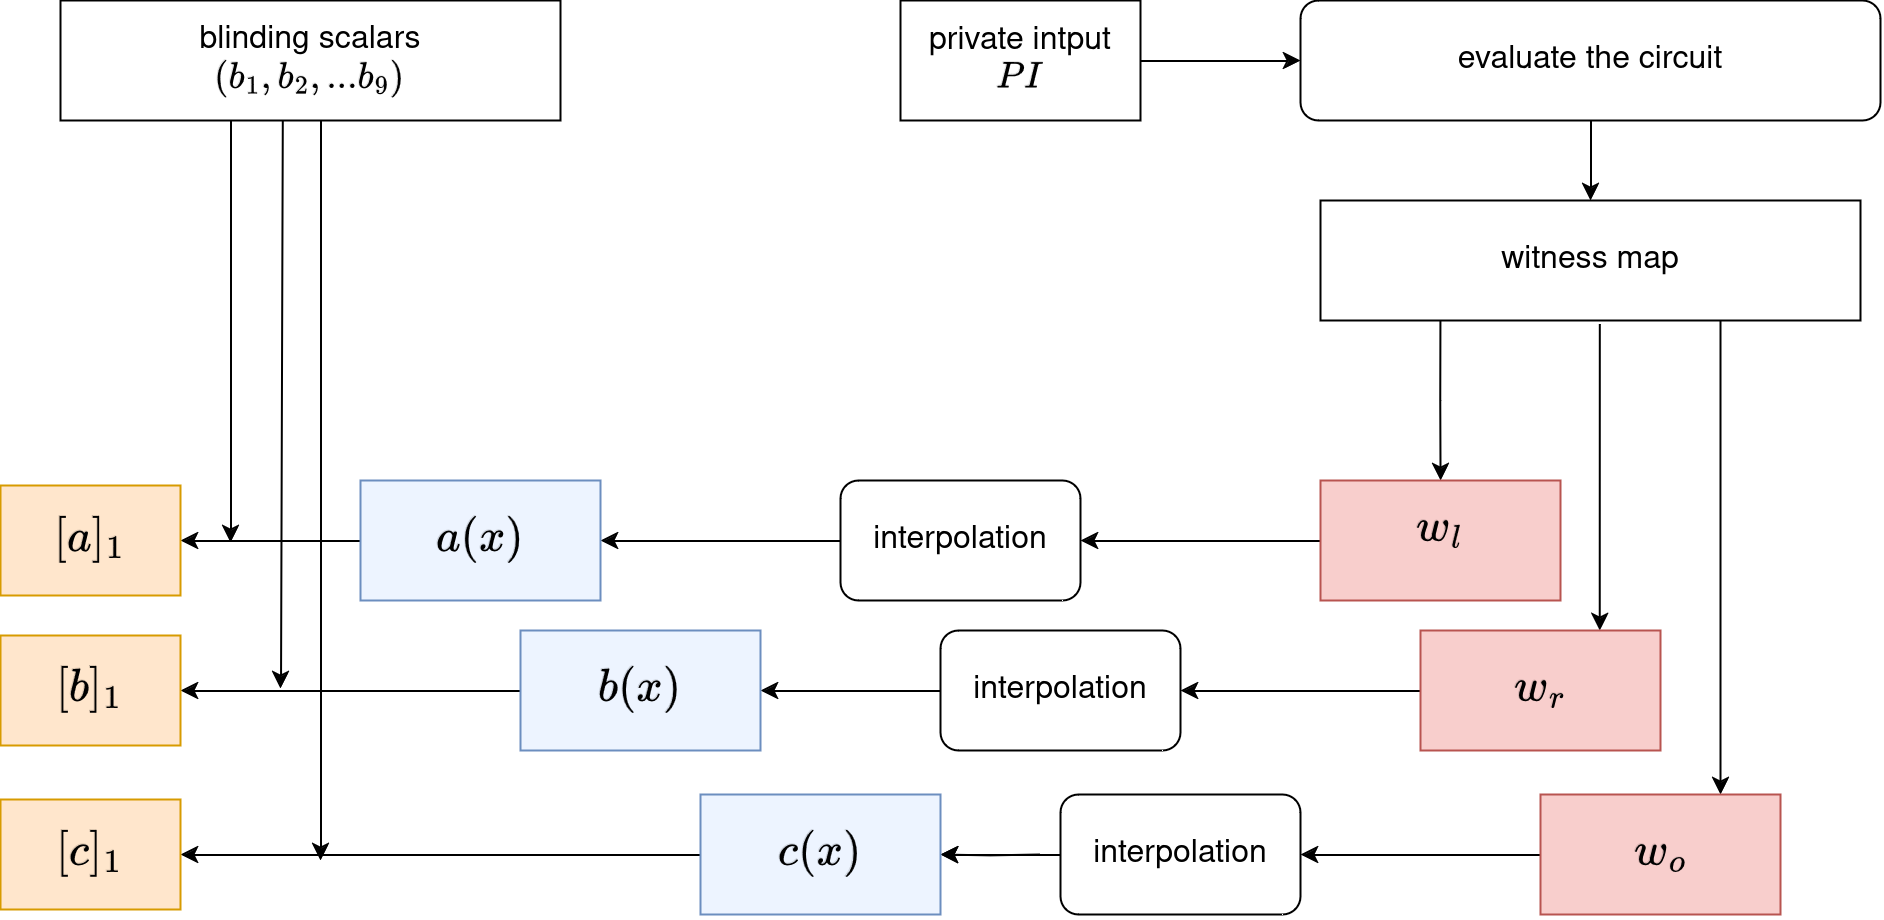
\includegraphics[width=1\linewidth]{round-figures/round1/round1.drawio.png}
    \caption{Round 1 Diagram}
\end{figure}


% \begin{note}[Intuition on why does this maintain the zero-knowledge property?]
%     Assume that the challenges for openings $z_1, z_2, \ldots, z_k$ are not in $H$ so $Z_H$ does not vanish on any of the challenges. The zero-knowledge (insanely informally) suggests that looking at the openings $p'(z_i)$ should give no information about $p(z_i)$. To the verifier openings, $p'(z_i)$ should look like uniformly randomly selected numbers. If there was any pattern in the openings the pattern might provide some (perhaps useful) information about the secret polynomial $p$. 

%     Take $b_1 + b_2x + b_2x^2 ... + b_{k+1}x^{k}$ as a blinding polynomial. Then the opening polynomial could be written as $p'(x) = b(x)Z_H + p(x)$. Now we notice that each set of openings $p'(z_1), p'(z_2), p'(z_3), \ldots p'(z_k)$ produces unique blinding polynomial. We take as a fact that a polynomial of degree $k$ is uniquely defined by $k+1$ points. This means that the polynomial $b(x)$ could be constructed by interpolating points: $\{(z_1, b(z_1)), (z_2, b(z_2)), (z_3, b(z_3)) \ldots, (z_k, b(z_k))\}$ form  $$b(z_i) = \frac{p'(z_i) - p(z_i)}{Z_H}$$

%     The last step is to realize that if we fix the secret polynomial $p(x)$ then by choosing the blinding polynomial we could get just about any set of opening points. Given that the coefficients of the blinding polynomial were chosen independently uniformly randomly we can say that the set of opening points $p'(z_1), p'(z_1), p'(z_1), \ldots, p'(z_k)$ produces also uniform distribution. Keep in mind that this trick only works if the blinding polynomial has a sufficient degree.
% \end{note}



\subsection{Computing wire polynomials}
Remember that we got the witness values in the arithmetization as columns of the computational table. The domain is chosen as $H = \{1, \omega, \omega^2, \ldots, \omega^{n-1}\}$ where $\omega^n = 1$. Choosing such a domain allows for a sparse representation of the vanishing polynomial as $Z_H(x) = x^n -1$ based on \cref{lemma:vanishing-poly}.

By pairing this domain with the witness $w$ we get the wire polynomials in the evaluation domain. To make commitments the polynomial needs to be in the coefficient form to evaluate it at the point $\tau$. Conversion to the coefficient form can be achieved by applying the Lagrange interpolation.

Finally, to make sure that the commitment to the wire polynomials does not leak information about the wire polynomial, they should be blinded. As described in \cref{theorem:blinding} this construction maintains the zero-knowledge property. The prover needs to uniformly randomly sample 9 blinding scalars $(b_1, b_2, \ldots, b_9)$. In round 1 there are sampled 9 blinding scalars, even though we only need 6. The remaining will be used in the next rounds.

\procedureblock[linenumbering]{$Round1_{\prover}$}{
    (b_1, \ldots, b_9) \sample \field^9 \\
    a(x) = (b_1x + b_2)Z_H(x) + \sum_{i=0}^{n-1} w_i L_i(x) \\
    b(x) = (b_3x + b_4)Z_H(x) + \sum_{i=0}^{n-1} w_{n+i} L_i(x) \\
    c(x) = (b_5x + b_6)Z_H(x) + \sum_{i=0}^{n-1} w_{2n+i} L_i(x) \\
    \pcreturn [a]_1, [b]_1, [c]_1
}


% ==============================================================================
% ===ROUND2=====================================================================
% ==============================================================================
\section{Round 2}
\label{chap:round2}

In this round awaits a big challenge - ensuring copy constraints of the circuit. We will see how it is possible to ensure the wiring constraints thanks to clever tricks. We will start by ensuring that constraints hold for inter-vector checks and then extend it to intra-vector checks.

Round overview:
\begin{enumerate}
    \item Receive permutation challenges $(\beta, \gamma) \in \field$ from the prover
    \item Compute permutation polynomial $z(x)$
    \item Compute and output commitment $[z]_1 \in \mathbb{G}_1$
\end{enumerate}

\begin{figure}[H]
    \centering
    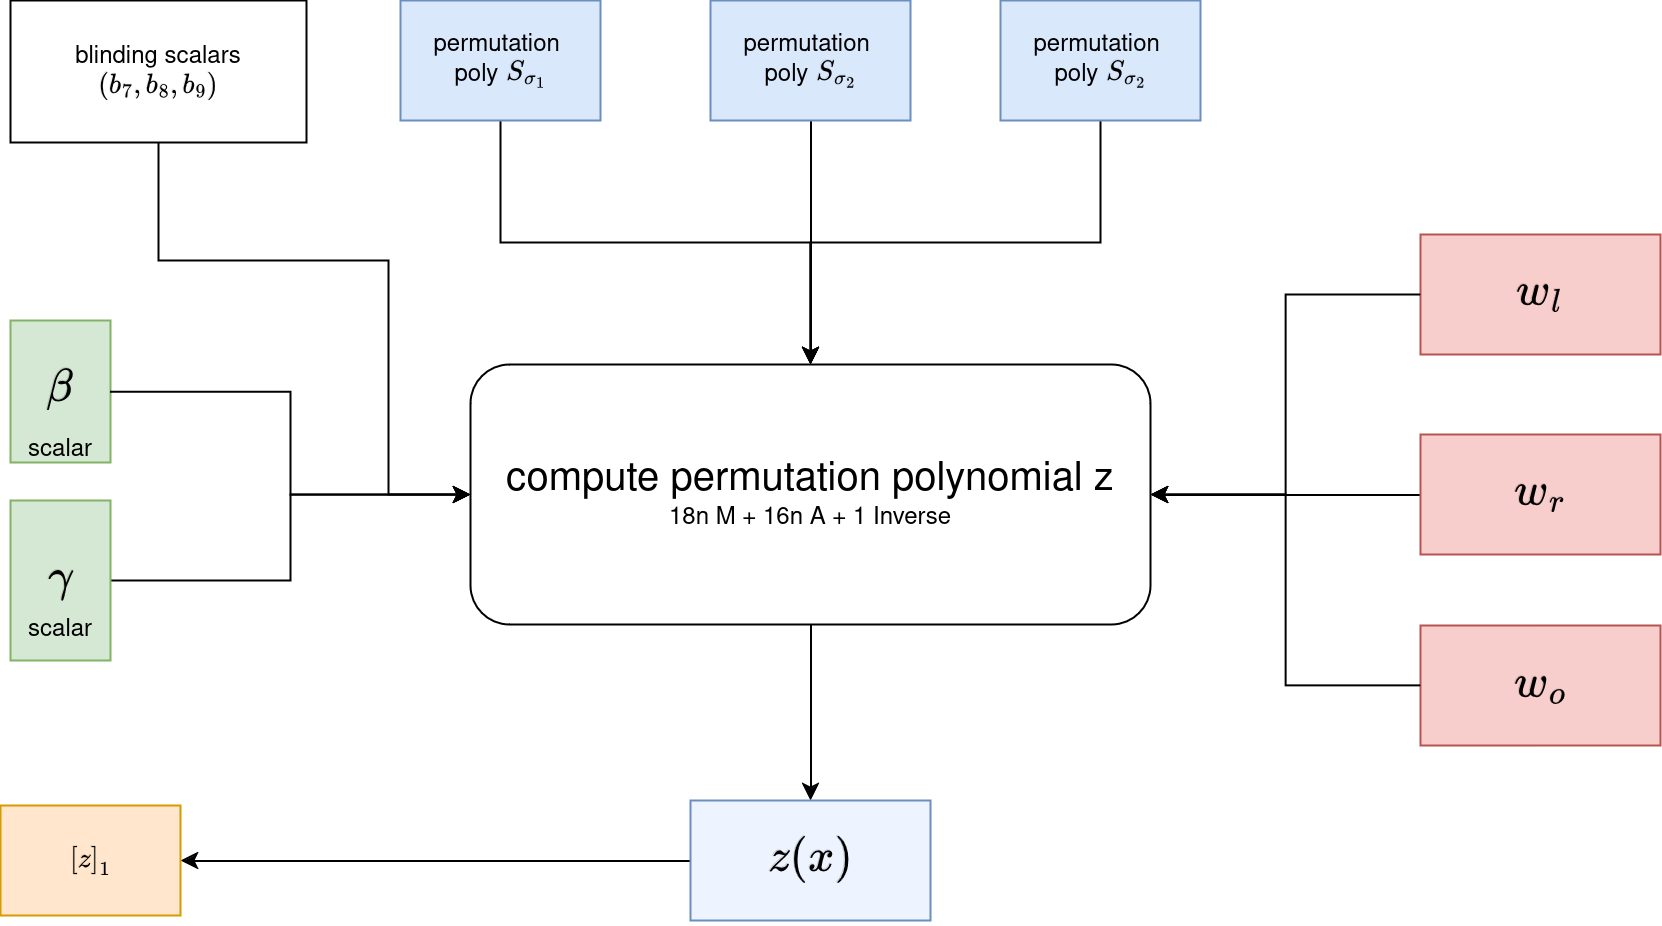
\includegraphics[width=1\linewidth]{round-figures/round2/round2.drawio.png}
    \caption{Round 2 Diagram}
    \label{fig:round2}
\end{figure}




\subsection{Intra-vector check}
We already know that the wire check could be efficiently checked by applying a suitable permutation function. Now we would like to show that this function indeed is a permutation and maintains the form of the vector. Given vectors $w$ and permutation function $\sigma$ we would like to efficiently verify that $\sigma$ is permutation. The brute-force approach has complexity $\bigO{n^2}$, on the other hand, naive approaches like performing sum checks are not reliable enough. Instead, the check could be performed by sampling uniformly random element $\beta$ and verifying $(w_1 + \beta)\ldots(w_n + \beta) \stackrel{?}{=} (\sigma(w_1) + \beta)\ldots(\sigma(w_n) + \beta)$. The trick is to think about these terms as polynomials with variable $\beta$, then we could use the theorem about polynomial intersection.

\begin{lemma}
    For vector $w$ of size $n$ and a function $\sigma$ of degree $n$ it is possible to verify that $\{w_1, w_2, \ldots, w_n\} \stackrel{?}{=} \{\sigma(w_1), \sigma(w_2), \ldots, \sigma(w_n) \}$ by $\prod_{i=0}^n (w_i + \beta) \stackrel{?}{=} \prod_{i=1}^n (\sigma(w_i) + \beta)$ with probability $\frac{n}{|\field|}$.
\end{lemma}

\begin{proof}
    Considering both $\prod_{i=0}^n (w_i + \beta) \text{and} \prod_{i=1}^n (\sigma(w_i) + \beta)$ as function in terms of $\beta$ they will have degree $n$ and thanks to the theorem about the number of the intersection \cref{theorem:poly-intersection} the probability of randomly hitting an intersection is $\frac{n}{|\field|}$.
\end{proof}

That looks promising. To use this check in the context of $\plonk$ we will be dealing with a tuple of field elements. The evaluation domain $H$ is set to be the $n$-th root of unity, so each point is in the form of tuple $(\omega^{i}, w_i)$ where $\omega^i \in H$. The permutation check is done very similarly but now we need to use two variables. Moreover, we need to change the image of the permutation function $\sigma_l: [1, 2, ... n] \rightarrow [1, \omega, \omega^2 ... \omega^n-1]$
$$\prod_{i = 1}^{n} w_i + \omega^{i-1} \beta + \gamma \stackrel{?}{=} \prod_{i = 1}^{n} w_i + \sigma_l(i) \beta + \gamma$$ 


The failure probability could be again determined by looking at the number of intersections of two polynomials. To show this formally we would again need to invoke the Schwartz-Zippel lemma but now for a multivariate case, \cite{MultivariateSZLemma}. Rephrasing this means that checking the statements shown below are equivalent except for negligible failure.

$$\{(\omega, w_{l_1}), (\omega^2, w_{l_2}), \ldots (\omega^{n-1}, w_{l_{n-1}})\} \stackrel{?}{=} \{(\omega, \sigma_l(1)), (\omega^2, \sigma_l(2)), \ldots (\omega^{n-1}, \sigma_l(n-1)\}$$
$$\iff$$
$$ 1 \stackrel{?}{=} \prod_{i = 1}^{n-1} \frac{w_i + \omega^i \beta + \gamma}{w_i + \sigma_l(i) \beta + \gamma}$$

From here on we could create a permutation polynomial for intra-vector case by interpolating below values over the domain $H$.

\begin{equation}
    \label{eq:intra-interpolation}
    (\frac{w_1 + \omega \beta + \gamma}{w_1 + \sigma_l(1) \beta + \gamma},
    \frac{(w_1 +  \omega \beta + \gamma)(w_2 + \omega^2 \beta + \gamma)}{(w_1 + \sigma_l(1) \beta + \gamma)(w_2 + \sigma_l(2) \beta + \gamma)}, \ldots,
    \prod_{i = 1}^{n-1} \frac{w_i + \omega^i \beta + \gamma}{w_i + \sigma_l(i) \beta + \gamma})
\end{equation}

This is great we have covered the core idea. Now we need to generalize this into inter-vector check and add blinding.

\subsection{Inter-vector check}
The first step in generalizing the previous inter-vector check is changing the permutation function. Remember the permutation function $\sigma^*$ from the setup? It will also implement rotation on equivalence classes of the circuit just on a different domain. Recall that the witness is composed of 3 columns of a computational trace table. The table has $n$ rows so the size of the witness $w$ would be $3n$. We can take the permutation function $\sigma: [1, 2, \ldots, 3n] \rightarrow [1, 2, \ldots, 3n]$. Now let's construct alternative domain $H' = H \cup (k_1H) \cup (k_2H)$, where $k_1, k_2 \in \field$ are chosen such that $H, k_1H, k_2H$ are distinct meaning $\forall p, q, r: \omega^p \neq \omega^q k_1 \neq \omega^r k_2$. The permutation function $\sigma^*$ will create mapping $[1, 2, \ldots, 3n] \rightarrow H'$ which means $i \rightarrow \omega^i, n+i \rightarrow k_1 \omega^i, 2n+i \rightarrow k_2 \omega^i$. Now we can construct functions:
$$f(i) = (w_{i} + \omega^i\beta + \gamma)(w_{n+i} + \omega^i\beta k_1 + \gamma)(w_{2n+i} + \omega^i\beta k_2+ \gamma)$$

\hl{the reason for using cosets is most probably to not get zero in the denominator}
\hl{explain how are the cosets constructed}

$$g(i) = (w_{i} + \sigma^*(i)\beta + \gamma)(w_{n+i} + \sigma^*(n+i \beta + \gamma)(w_{2n+i} + \sigma^*(2n+i)\beta + \gamma)$$

To perform an inter-vector check we would need to verify: $1 \stackrel{?}{=} \prod_{i=1}^{n-1} f(i) / g(i)$. This expression might be undefined when $g(i)$ is 0 however this only happens with negligible probability. But still, when it happens, the protocol will be aborted.

\subsection{The Permutation Polynomial}
Now we have all of the ingredients to construct the permutation polynomial. In this section, we will only show how to compute it. In the following round, the prover also has to convince the verifier that this polynomial was computed correctly. The permutation polynomial is defined as follows:

\begin{definition}[Permutation polynomial]
    $$
    z(x) = 
    \begin{cases} 
          1 & x = \omega \\
          \prod_{j=1}^{i-1} \frac{f(j)}{g(j)} & x = \omega^i \text{ where } i \in \{2, 3, \ldots, n\}
    \end{cases}
    $$
\end{definition}

Again, we are taking the product of ratios, where the numerator represents the former set and the denominator represents the permuted set. If each of these ratios is 1 that means the permutation did not change the set.

How do we construct this polynomial? We will proceed as usual and perform Lagrange interpolation of these values:
$$\frac{f(1)}{g(1)}, \frac{f(1)f(2)}{g(1)g(2)}, \frac{f(1)f(2)f(3)}{g(1)g(2)g(3)}, \ldots, \prod_{i=1}^{n-1} \frac{f(i)}{g(i)}$$

That means the almost final permutation polynomial could be written as:
$$\Tilde{z}(x) = \sum_{i=1}^{n-1} L_{i+1}(x) \prod_{j=1}^i \frac{f(i)}{g(i)}$$

Notice that this polynomial will be zero on $\omega$ because in the sum there are langrange basis $(L_2(x), L_3(x), \ldots, L_n(x))$. To enforce that the permutation polynomial evaluates to 1 on $\omega$ we add Lagrange basis $L_1(x)$ to $\Tilde{z}(x)$. To finish it up just add blinding scalars but this time we will need a blinding polynomial of degree 2 because later there will be two openings of $z$ (in $W_{\challenge}(x), W_{\challenge\omega}(x)$).

\begin{equation}
    z(x) = (b_7x^2 +b_8x +b_9)Z_H(x) + L_1(x) + \Tilde{z}(x)
\end{equation}

\procedureblock[linenumbering]{$Round2_{\prover}$}{
    \beta, \gamma \gets H \\
    z(x) = (b_7x^2 +b_8x +b_9)Z_H(x) + L_1(x) + \Tilde{z}(x) \\
    \pcreturn [z]_1
}



% ==============================================================================
% ===ROUND3=====================================================================
% ==============================================================================
\section{Round 3}
\label{chap:round3}

In the previous rounds we have created some constraints now it is time to aggregate them. The prover needs to combine these checks as well as convince the prover that the permutation polynomial was computed as it is specified by the protocol. But that is not all we also need to handle the problem with polynomials exceeding the degree bound $n$. 

\begin{figure}[H]
    \centering
    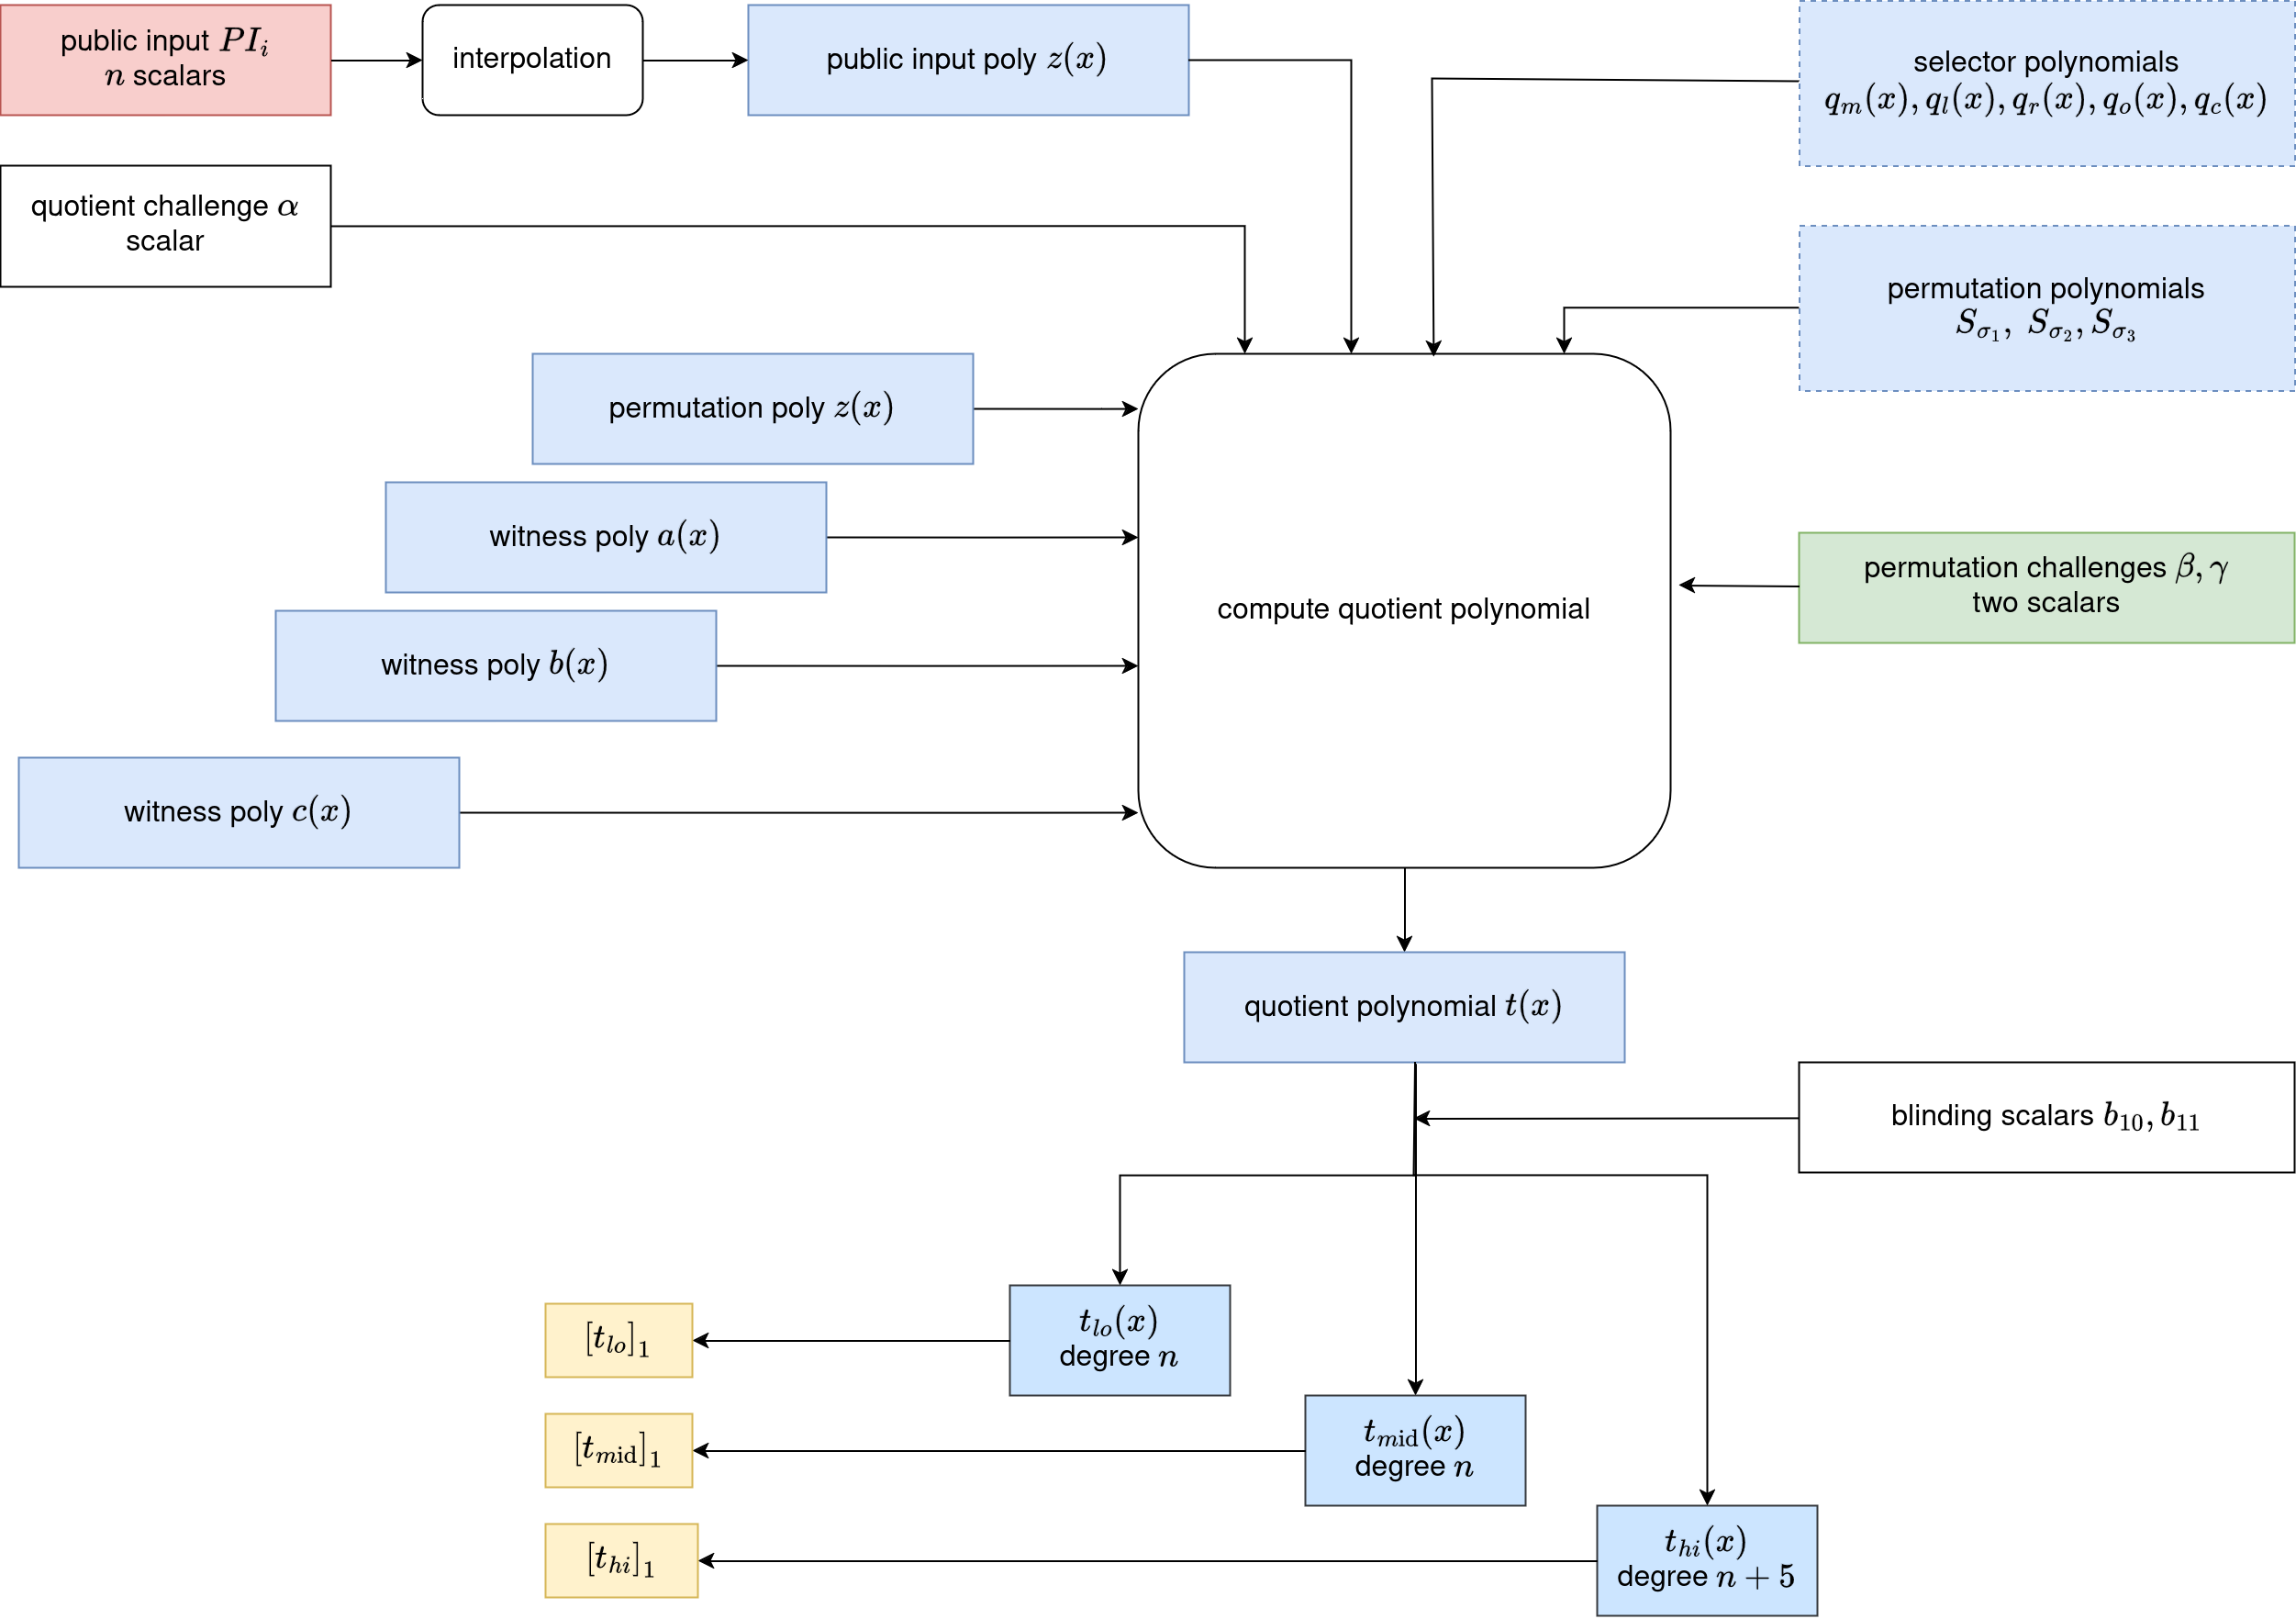
\includegraphics[width=1\linewidth]{round-figures/round3/round3.drawio.png}
    \caption{Enter Caption}    
\end{figure}


In the last round we have computed and committed to $z(x)$ however, we did not prove that it was computed correctly. Specifically we have promised that $z(\omega) = 1$, otherwise for $x = \omega^i$ it is cumulative product $\prod_{j=1}^i f(i) / g(i)$. This is the same as checking:

\begin{enumerate}
    \item $(z(x)-1)L_1(x) = 0$
    \item $z(x)f'(x) = g'(x)z(x\omega)$
\end{enumerate}

$$\Tilde{f}(x) = (a(x) + x \beta + \gamma)(b(x) + x \beta k_1+ \gamma)(c(x) + x \beta k_2+ \gamma)$$
$$\Tilde{g}(x) = (a(x) + \beta S_{\sigma_1}(x) + \gamma)(b(x) + \beta S_{\sigma_2}(x)+ \gamma)(c(x) + \beta S_{\sigma_3}(x) + \gamma)$$

This is not immediately obvious and we will try to show it shortly


In this blog we will not be constructing the quotient polynomial from the bottom. First we will introduce the quotient polynomial in it's full beauty and then dissect it. The quotient polynomial denoted as $t(x)$ in the paper consist of sum of 3 expressions 
$t = t_1 + t_2 + t_3$:
\begin{equation}\label{quotient1}
    t_1(x) = (a(x)q_{l}(x) + b(x)q_{r}(x) + c(x)q_{o}(x) + a(x)b(x)q_{m}(x) + PI(x) + q_{c_i})\frac{1}{Z_H(x)}
\end{equation}

\begin{equation}\label{quotient2}
    t_2(x) = (f'(x)z(x))\frac{\alpha}{Z_H(X)} - (g'(x)z(\omega x))\frac{1}{Z_H(x)}
\end{equation}

\begin{equation}\label{quotient3}
    t_3(x) = (z(x)-1)L_1(x\frac{1}{Z_H(x)}
\end{equation}

$$t(x) = t_1(x) + t_2(x) \alpha + t_3(x) \alpha^2$$

The quotient polynomial might be long but it is composed of elements that pretty much make sense. So let's just work through it.

\subsection{Computing quotient polynomial}

\subsubsection{3rd term}
This corresponds to checking the first part of definition of $z(x)$. So let's prove it is correct: 
\begin{theorem}[First property of permutation polynomial]
    $\forall x \in H: (z(x)-1)L_1(x) = 0 \implies z(\omega) = 1$
\end{theorem}

\begin{proof}
    For $x \neq \omega$ the Lagrange basis evaluate to 0 and there is not any constraint for $z(x)$. However for $x = \omega$ we get $z(\omega) - 1 = 0$ meaning that $z(\omega)$ indeed must be equal to 1.
\end{proof}

\subsubsection{2nd term}
\begin{theorem}[First property of permutation polynomial]
    $\forall i \in [n]: z(\omega^i)f'(\omega^i) = g'(\omega^i)z(\omega^{i+1}) \implies \forall i \in [n]: z(\omega^i) = \prod_{j=1}^{i-1} \frac{f'(\omega^j)}{g'(\omega^j)}$
\end{theorem}

\begin{proof}
    We will show this by induction. For the base case $i=1$ we get:
    $$z(\omega)f(\omega) = g(\omega)z(\omega^2)$$
    $$z(\omega^2) = \frac{f(\omega)}{g(\omega)}$$
    We know that $z(\omega) = 1$ there is already check for that, the rest simplifies easily. For the case $i =k+1$
    $$z(\omega^{k+1})f(\omega^{k+1}) = g(\omega^{k+1})z(\omega^{k+2})$$
    $$\prod_{j=1}^k \frac{f(\omega^j)}{g(\omega^j)} f(\omega^{k+1}) = g(\omega^{k+1})z(\omega^{k+2})$$
    $$\prod_{j=1}^k \frac{f(\omega^j)}{g(\omega^j)} \frac{f(\omega^{k+1})}{g(\omega^{k+1})} = z(\omega^{k+2})$$
    $$z(\omega^{k+2}) = \prod_{j=1}^{k+1} \frac{f(\omega^j)}{g(\omega^j)}$$    
\end{proof}


\subsubsection{1st term}
This might feel familiar and in fact it very much should. These are the gate constraints introduced in the overview \eqref{chap:arithmetization}. Including them in the quotient polynomial makes sure that they indeed hold for each gate. 

Each of the check pass if the designated polynomial is zero on the evaluation domain. We would like to combine like to batch these checks such that $t(x) = 0 \iff t_1(x) = 0 \wedge t_2(x) = 0 \wedge t_3(x) = 0$. To achieve this we will construct the quotient polynomial as:
$$t(x) = t_1(x) + t_2(x)\alpha + t_3(x)\alpha^2$$

Why does this work? The set $\forall \alpha \in \field \{1, \alpha, \alpha^2\}$ is linearly independent:
$$a + b\alpha + c\alpha^2 = 0 \iff a = b = c = 0 $$

To see this let's first assign $\alpha = 0$ which implies that $a = 0$. Now we are left with $b\alpha + c\alpha^2 = 0$. Now we can pick we make following assignment:
$$\alpha = 1: b + c = 0$$
$$\alpha = 1^{-1}: -b + c = 0$$
$$b+c -b +c = 0$$

Here we get that $c = 0$ which means that $b$ also needs to be 0.


\subsection{Splitting quotient polynomial}

Now we can finally construct the quotient polynomial $t(x)$. However, the problem is that the degree of the polynomial is too big. We want our polynomials to have the maximum degree of $n$ to be able to commit to them. We assumed so in the setup while creating SRS and the whole KZG commitment scheme relies on it. We can split $t(x)$ into $< n$ degree polynomials $t_{lo}'(x), t_{mid}'(x)$ and $t_{hi}'(x)$ of degree at most $n+5$ such that: $$t(x) = t_{lo}'(x) + x^nt_{mid}'(x) + x^{2n}t_{hi}'(x)$$

Why $t_{hi}$ has degree bound $n+5$? Look just at $t_2$ where we multiply $\Tilde{f}(x)z(x)$. The degree of $\Tilde{f}(x)$ is $3(n+1)$ because of each of $a(x), b(x), c(x)$ have degree of $n+1$ since they interpolate $n$ points. The permutation polynomial has degree $n+2$ which makes it $4n+5$ and then division by $Z_H$ with degree $n$ resulting in $3n+5$.


How can we split the quotient polynomial? We simply compute the quotient polynomial and take $c_0 + c_1x + c_2x^2 + ... + c_n x^n $ as polynomial $t_{lo}$. Then take $c_{n+1}x^{n+1} + c_{n+2}x^{n+2} + ... + c_{2n}x^{2n}$ divide it by $x^n$ and create $t_{mid}$ with degree $n$. Then we do a similar thing for $t_{hi}$ but divide it by $x^{2n}$.
$$t(x) = t_{lo}(x) + x^n t_{mid}(x) + x^{2n}t_{hi}(x)$$

Nice this looks better, but we also need to blind them. $b_{10}, b_{11} \in \field$ and use them as follows: $t_{lo}(x) = t_{lo}'(x) + b_{10}x^n , t_{mid}(x) = t_{mid}'(x) - b_{10} + b_{11}x^n, t_{hi}(x) = t_{hi}'(x) - b_{11}$. Now we are ready to calculate commitments with degree at most $n+5$: $[t_{lo}(s)]_1, [t_{mid}(s)]_1, [t_{hi}(s)]_1$.

\procedureblock[linenumbering]{$Round3_{\prover}$}{
    \alpha \sample \field \\
    t(x) =  t_1(x) + t_2(x) \alpha + t_3(x) \alpha^2 \\
    t(x) -> t_{lo}, t_{mid}, t_{high} \\
    \pcreturn [t_{lo}]_1, [t_{mid}]_1, [t_{high}]_1 \\
}

% ==============================================================================
% ===ROUND4=====================================================================
% ==============================================================================
\section{Round 4}
\label{chap:round4}

\begin{enumerate}
    \item Compute evaluation challenge $\challenge \in \field = \challenge$
    \item Compute and output opening evaluations $\overline{a}, \overline{b}, \overline{c}, \overline{z_\omega}, \overline{S}_{\sigma_1}, \overline{S}_{\sigma_2}$
\end{enumerate}

\begin{figure}[H]
    \centering
    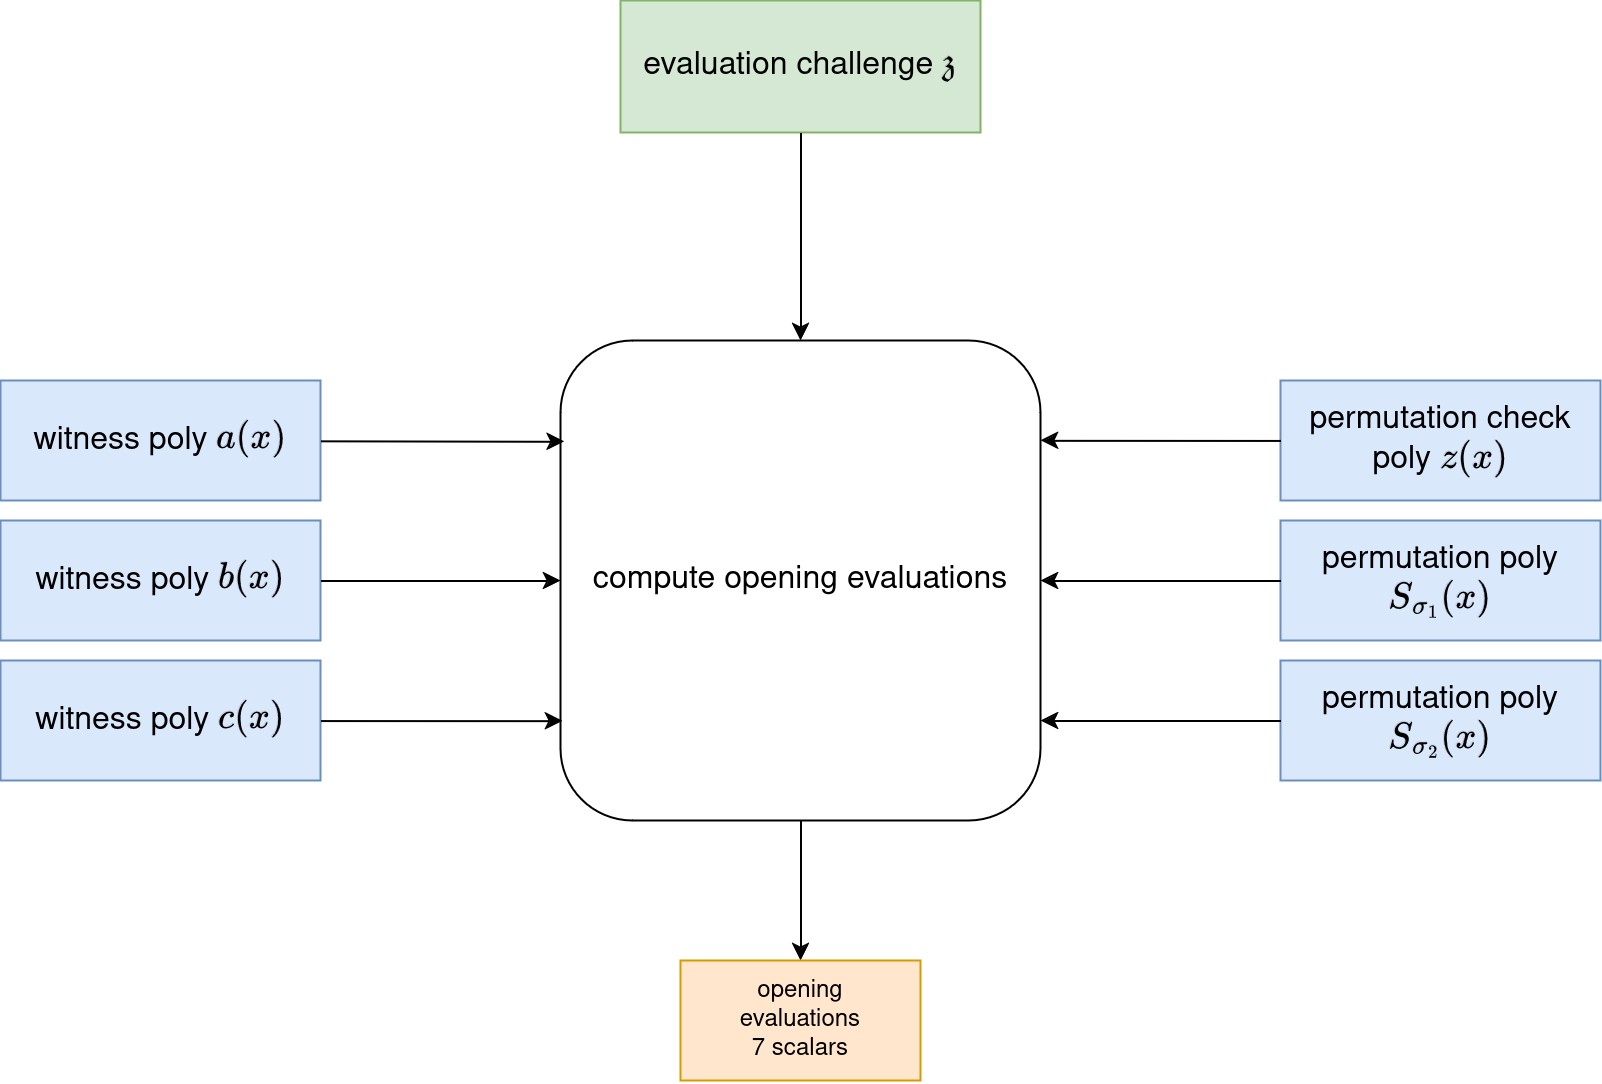
\includegraphics[width=1\linewidth]{round-figures/round4/round4.drawio.png}
    \caption{Enter Caption}
    
\end{figure}

In this round the prover computes evaluation opening, know in the business as linearisations, which are denoted with a horizontal line above. The openings are performed at a random point $\challenge$. In interactive case $\challenge$ is chosen by the verifier, here it is given by a hash function applied to transcript of the prover computation. All the prover has to do is calculate and output: $\overline{a} = a(\challenge), \overline{b} = b(\challenge), \overline{c} = c(\challenge), \overline{z_\omega} = z(\omega\challenge),\overline{S}_{\sigma_1} = S_{\sigma_1}(\challenge), \overline{S}_{\sigma_2} = S_{\sigma_2}(\challenge)$. Is is as simple as that. Now let's look at a way to minimize number of opening to minimize protocol communication costs.

\subsection{Linearization trick}
Imagine that the prover wants to show that $h_1(x)h_2(x) - h_3(c) = 0$ over a specified domain. Then he sure needs to commit to each to these polynomials and send their openings at a random point $\challenge$, resulting in 3 commitments and 3 openings. Verifier needs to check $\forall x \in H: h_1(x)h_2(x) - h_3(c) = 0$ which thanks to \href{https://en.wikipedia.org/wiki/Schwartz%E2%80%93Zippel_lemma}{Schwartz-Zippel} simplifies to checking just at a single random point $\challenge$. 

There is a better approach, utilizing the linearisation polynomial $l(x) = \overline{h}_1 h_2(x) - h_3(x)$ which as usual evaluates to zero over the domain $H$. As before the prover needs to send commitments $[h_1]_1, [h_2]_1, [h_3]_1$. However now he will send only 2 openings of $\overline{h_1} = h_1(\challenge)$ and $\overline{l} = l(\challenge) = \overline{h_1}h_2(\challenge) - h_3(\challenge)$. Notice that the number of the commitments stays the same because the verifier can calculate $[l]_1 = \overline{h}_1[h_2]_1 + [h_3]_1$. This is possible because commitments are additively homomorphic. The verifier checks that $l(\challenge) = 0$ which is equivalent to $h_1(\challenge)h_2(\challenge) - h_3(\challenge) = 0$ from how we defined $l(x)$. Keep in mind there is not anything complex, you can see the difference in the comparison below. The left diagram has 3 opening and the right one is the modified one with 2 opening and the linearisation polynomial.

\begin{figure}[H]
    \centering
    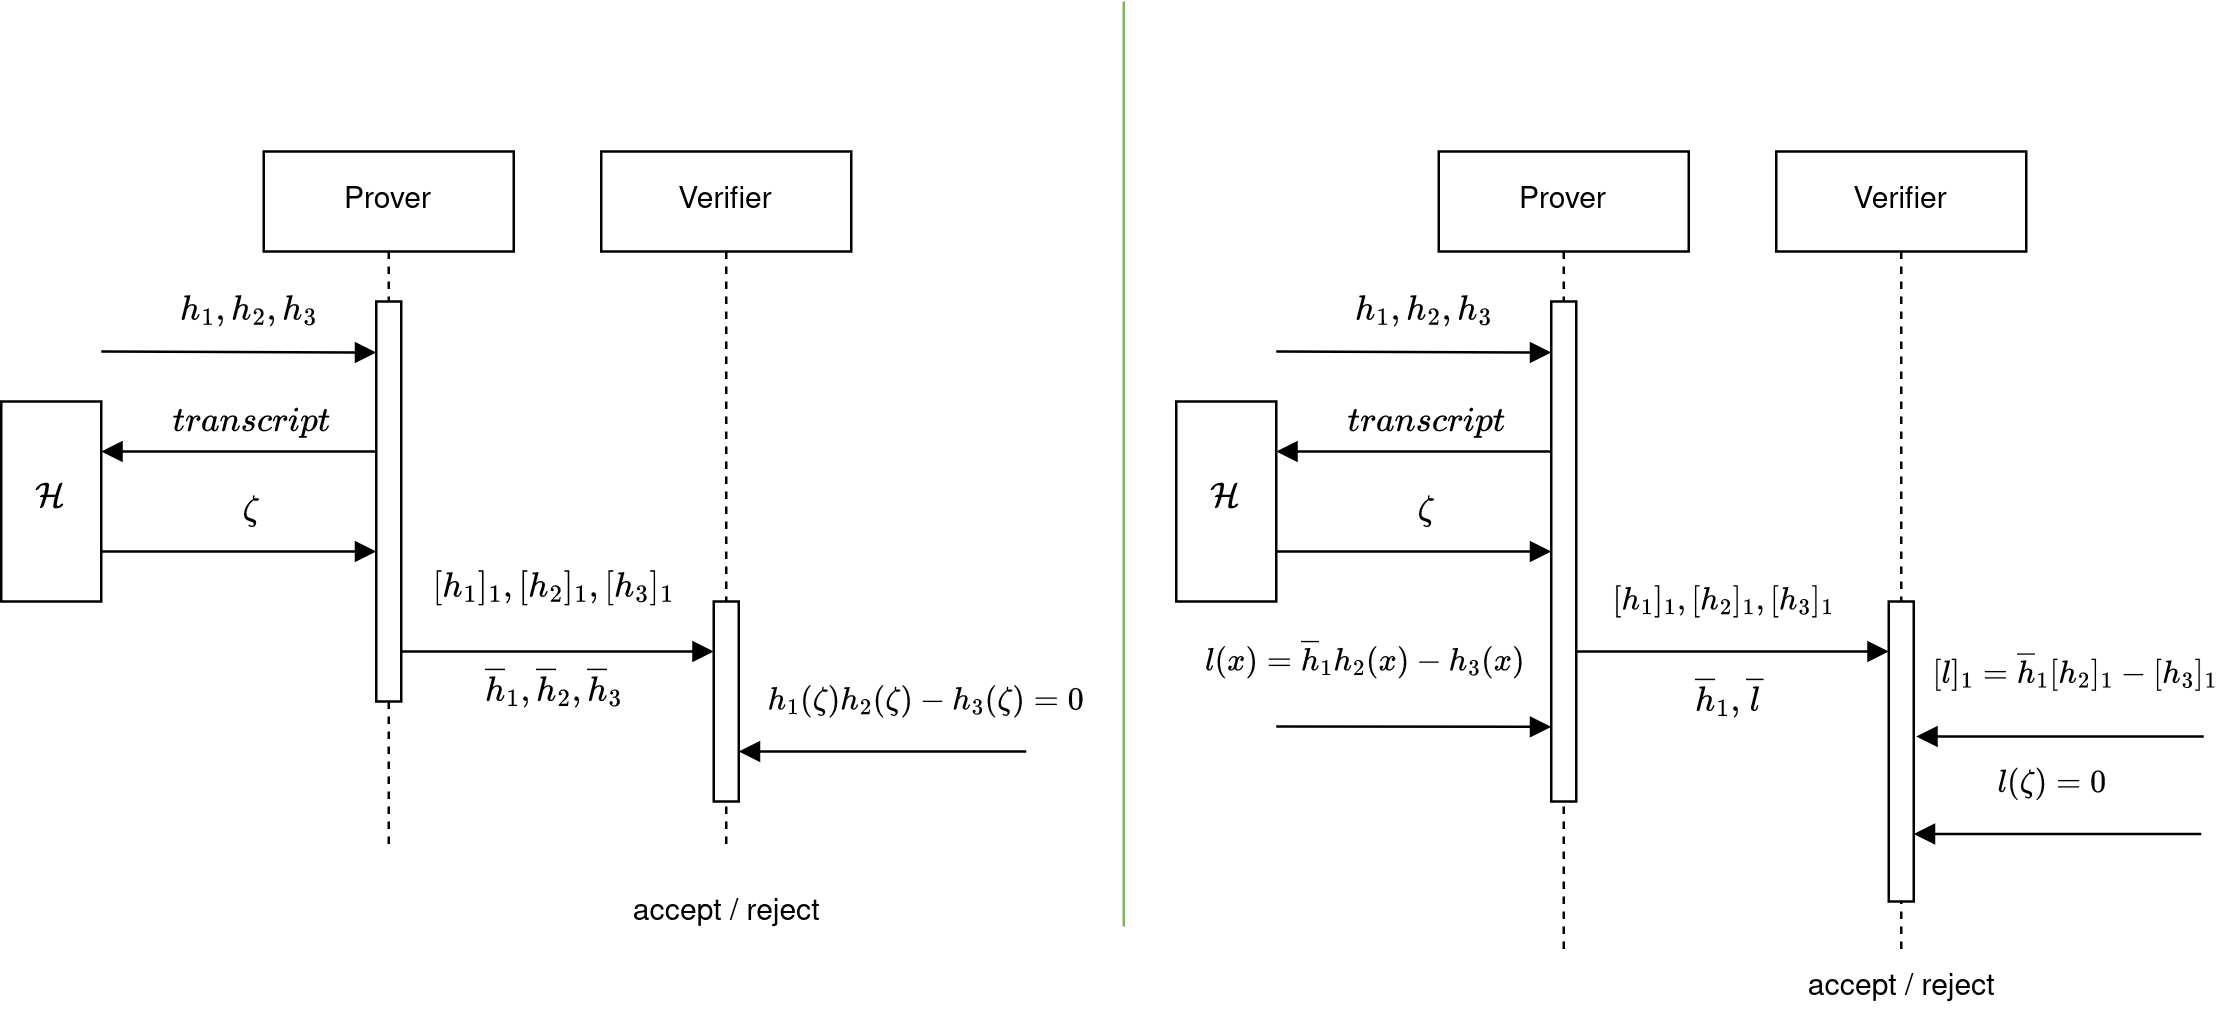
\includegraphics[width=1\linewidth]{round-figures/round4/linearisation_trick.drawio.png}
    \caption{Linearization trick}
\end{figure}

Why do we need to send $\overline{h}_1$?
Elliptic curve pairing which are not homomorphic for multiplication, meaning we cannot multiply to commitments so it is not possible to compute commitment to $l$ as $[l]_1 = [h_1]_1[h_2]_1 - [h_3]_1$. By sending $\overline{h}_1$ we can calculate the multiplication $\overline{h}_1[h_2]_1$ since here we perform multiplication by opening which is effectively a constant.

The linearisation trick is the reason why we are not sending evaluation at $\challenge$ for selector polynomials $q_l(x), q_r(x), q_m(x), q_c(x)$, permutation function $S_{\sigma_3}$ and permutation $z(x\omega)$ in the following round. That already is a significant improvement. If you are asking why do we need $z(x\omega)$ it is to check for 2. part of definition for the permutation polynomial $z(x)$.

\procedureblock[linenumbering]{$Round4_{\prover}$}{
    \challenge \\
    \overline{a} = a(\challenge), \overline{b} = b(\challenge), \overline{c} = c(\challenge), \overline{z_\omega} = z_\omega(x), \overline{S}_{\sigma_1} = S_{\sigma_1}(x), \overline{S}_{\sigma_2} = S_{\sigma_2}(x) \\
    \pcreturn \overline{z_\omega}, \overline{S}_{\sigma_1}, \overline{S}_{\sigma_2}
}

% ==============================================================================
% ===ROUND5=====================================================================
% ==============================================================================
\section{Round 5}
\label{chap:round5}

Previously we have seen how to perform linearisation trick to minimize the number of openings. We will use this knowledge in the grand finale of the prover algorithm. Here all of the constraints will be combined to generate the proof $\pi$ which will be sent to the verifier.

\begin{enumerate}
    \item Compute opening challenge $v \in \field$
    \item Compute linearisation polynomial $r(x)$
    \item Compute opening proof polynomial $W_{\challenge}(x)$
    \item Compute opening proof polynomial $W_{\challenge\omega}(x)$
    \item Return proof $\pi$
\end{enumerate}

\begin{figure}[H]
    \centering
    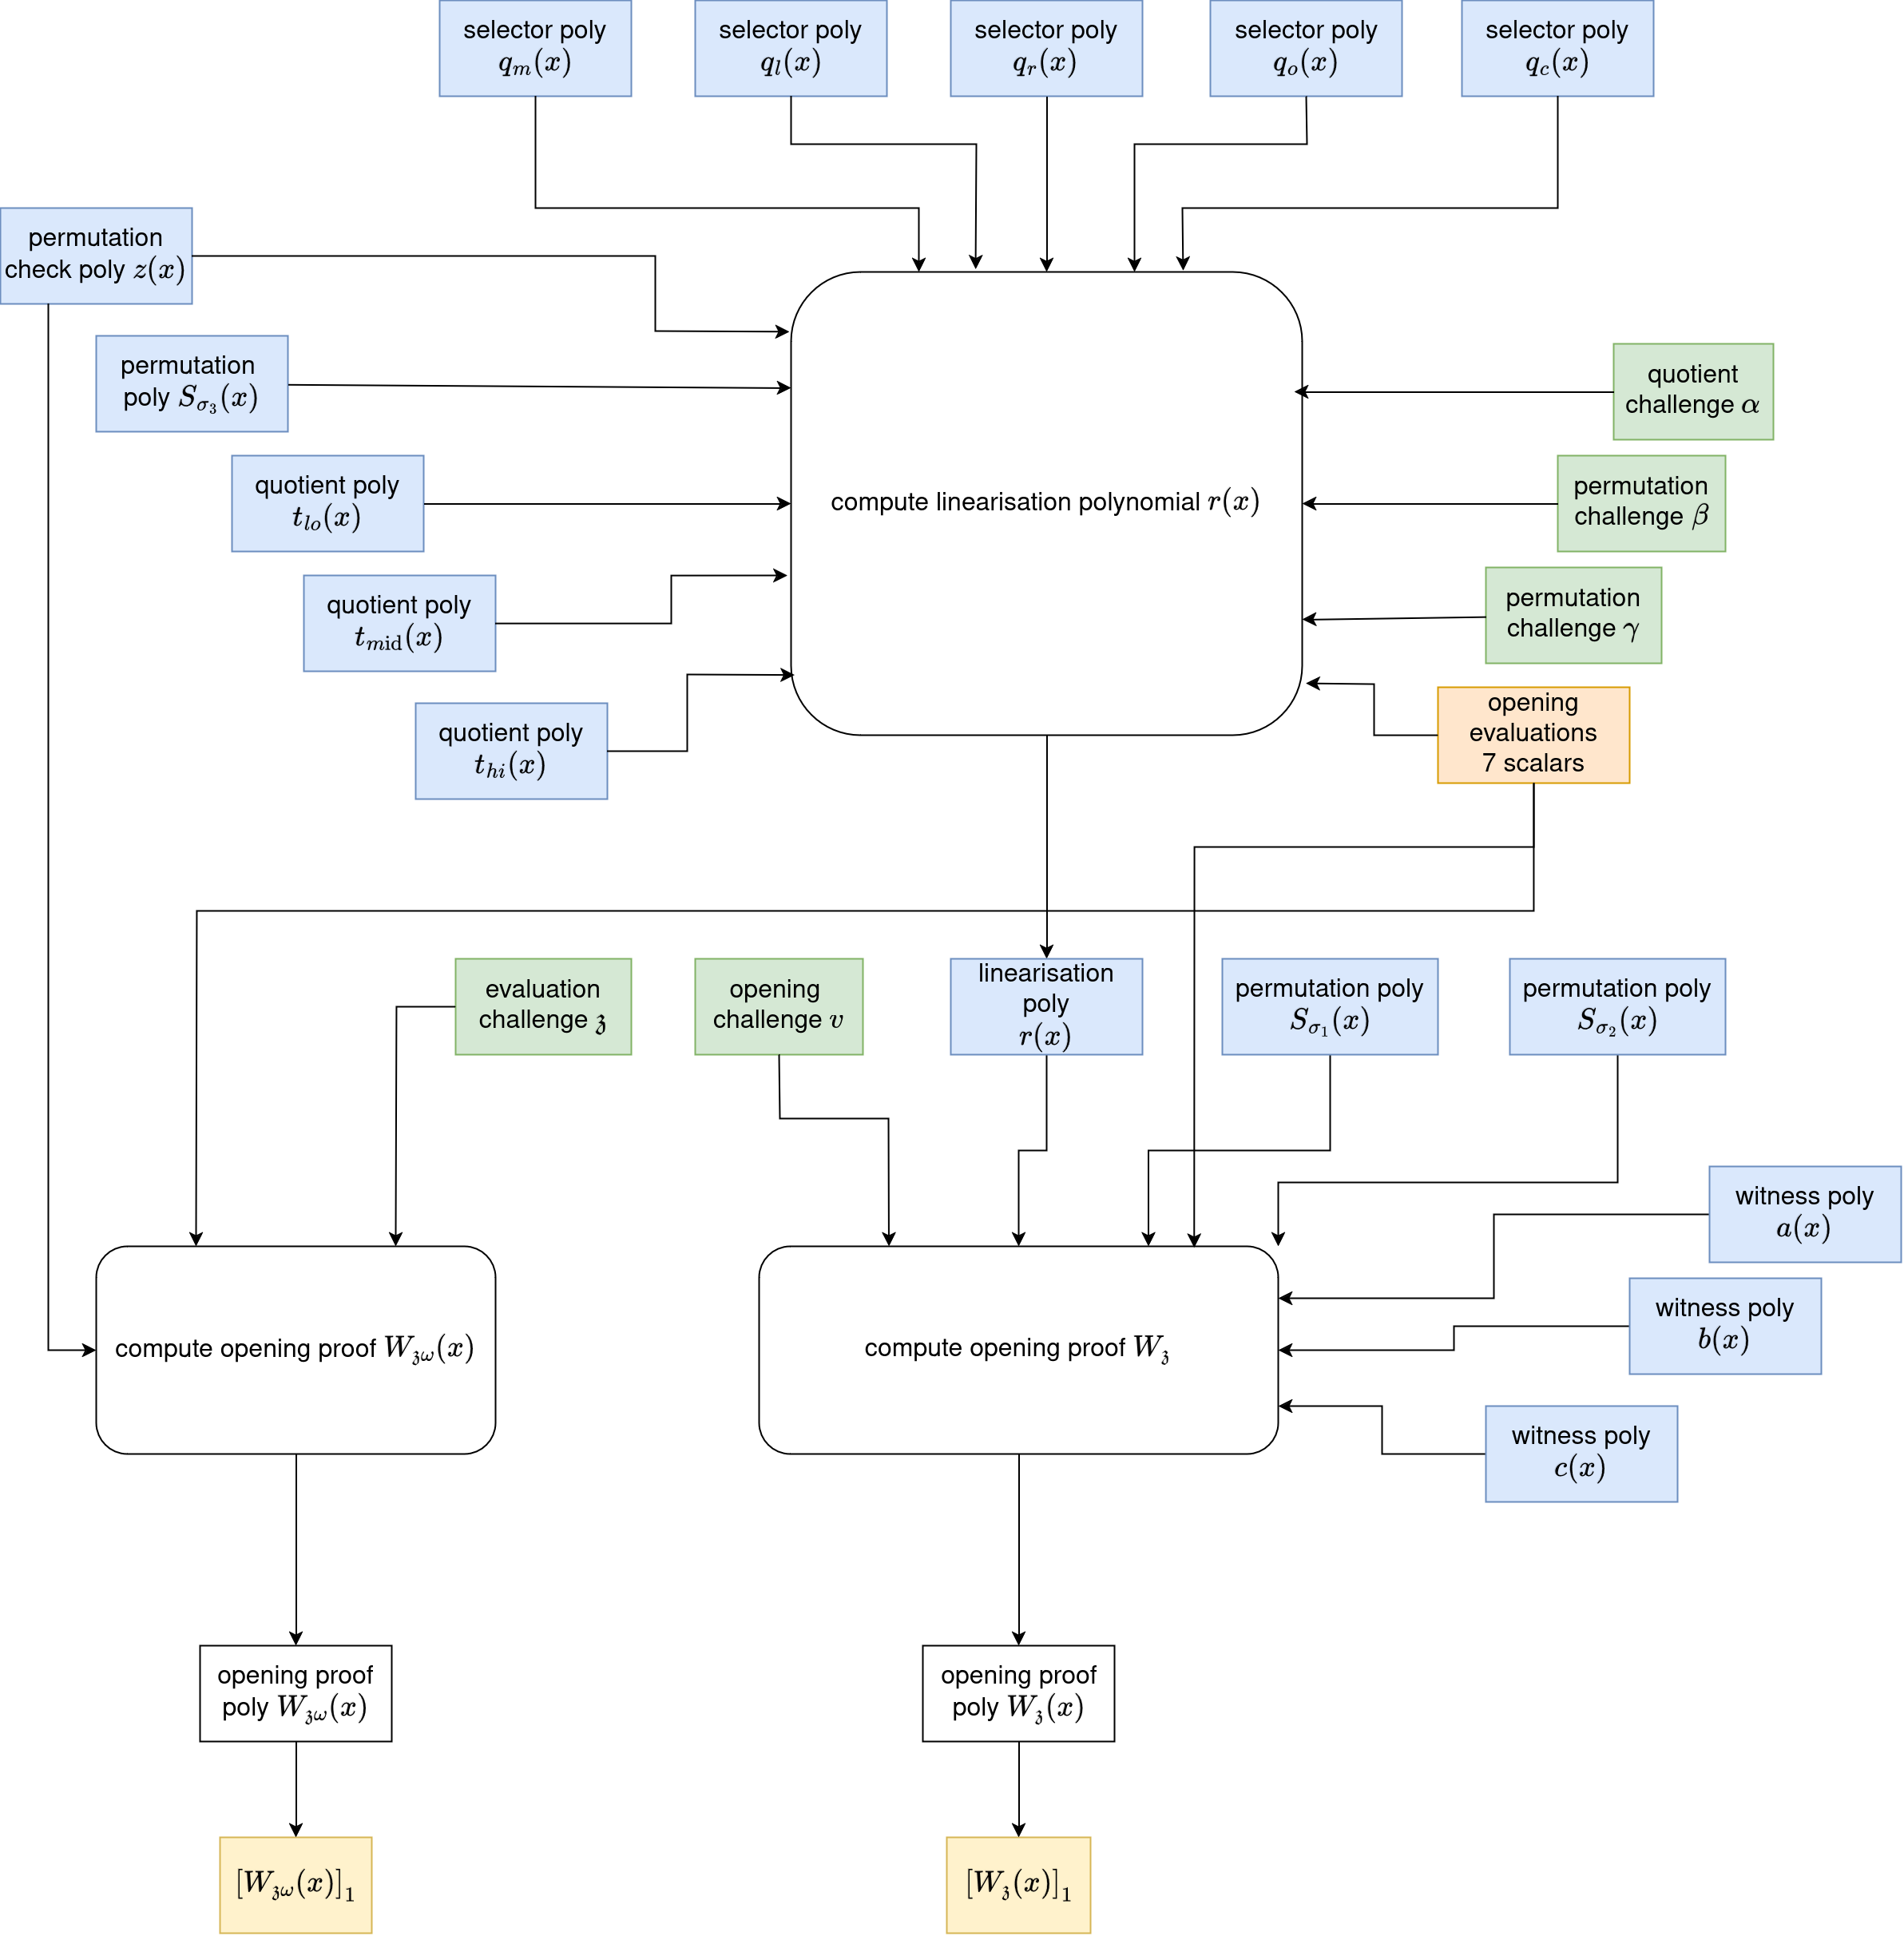
\includegraphics[width=1\linewidth]{round-figures/round5/round5.drawio.png}
    \caption{Enter Caption}
    
\end{figure}

\subsection{Linearisation polynomial}
Prover computes linearisation polynomial $r(x)$ which is a linear combination of all commitments. This polynomial is created using the evaluations from the round 4. Recall from the third round: 
\begin{equation}\label{pseudo-linearisation-poly}
    t_{lo} + x^{n}t_{mid}(x) + x^{2n}t_{hi} = t(x) = \frac{s(x)}{Z_H(x)}
\end{equation}

We know that the quotient polynomial should evaluate to zero over the domain $H$, therefore needs to exists a polynomial $s$ for which above holds. From that we can construct the linearisation polynomial:
$$r(x) = s(x) - Z_H(\challenge)(t_{lo}(x) + \challenge^n t_{mid}(x) + \challenge^{2n}t_{hi}(x)$$

Notice that this polynomial is just rewritten \eqref{pseudo-linearisation-poly} from which follows that it should be zero when evaluated at the point $\challenge$. In the full form the quotient polynomial could be written as:

\begin{multline}
    r(x) = [\overline{a}\overline{b}q_m(x) + \overline{a}q_l(x) + \overline{b}q_r(x) + \overline{c}q_o(x) + PI(\challenge) + q_c(x)] \\
    + \alpha [
        (\overline{a} + \beta \challenge + \gamma)(\overline{b} + \beta k_1 \challenge + \gamma)(\overline{c} + \beta k_2 \challenge + \gamma)z(x) \\
        - (\overline{a} + \beta \overline{s}_{\sigma_1} + \gamma)(\overline{b} + \beta \overline{s}_{\sigma_2} + \gamma)(\overline{c} + \beta S_{\sigma_3}(x) + \gamma)\overline{z}_{\omega}
    ] \\
    + \alpha^2 [(z(x) -1)L_1(\challenge)] \\
    - Z_H(\challenge)(t_{lo}(x) + \challenge^n t_{mid}(x) + \challenge^{2n} t_{hi}(x))
\end{multline}

Here the polynomial $s$ is substituted by the \textit{gate check} + \textit{1. permutation check} + \textit{2. permutation check}. It is good to notice which variables are linearised. They are the ones without the horizontal line: $q_m, q_l, q_r, q_o, q_c, z, S_{\sigma_3}$. This is determined by the linearization trick described in the previous post \eqref{chap:round4}. After you understand why those could be linearized and others not make sure to understand that the prover is able to calculate the commitment to $r(x)$ from the proof $\pi$ at the end of this post. 

\subsection{Opening proof polynomial}

\subsubsection{First opening proof polynomial}
Prover calculates $W_{\challenge}(x)$ the opening proof polynomial to verify that linearisation polynomial $r(x) = 0$ over $H$, by opening a single evaluation $\challenge$. This a form of aggregation and is essentially the same as checking that each of the constraints obtained in $r(x)$ evaluate to 0. Besides the verifier also needs to check for correctness of $a(x), b(x), c(x), S_{\sigma_1}(x), S_{\sigma_2}(x)$. These are combined into linearly independent set using $(1, v, v^2, v^3, v^4, v^5)$ where $v \in \field$ is given from $\mathcal{H}(transcript)$. Linear independence is used for similar reason as in the quotient polynomial.

\begin{multline}
    W_{\challenge}(x) = \frac{1}{x - \challenge} (
        r(x) 
        + v(a(x) - \overline{a})) 
        + v^2(b(x) - \overline{b})) \\
        + v^3(c(x) - \overline{c})) 
        + v^4(S_{\sigma_1}(x) - \overline{S}_{\sigma_1})) 
        + v^5(S_{\sigma_2}(x) - \overline{S}_{\sigma_2})) 
\end{multline}

The prover needs to show that all of the terms are divisible by $x - \challenge$ meaning that $\challenge$ is a root for each of them.

Let's be a bit more specific about previous check
If $x - \challenge$ divides a polynomial, in our case $r(x)$, that means there needs to exist $s(x)$:
$$\frac{r(x)}{z-\challenge} = s(x)$$
$$r(x)= s(x)(x-\challenge)$$
That means $r$ has $\challenge$ as root. The rest of the polynomials are in the form: $(p(x) - \overline{p})$. The check essentially says: if $x - \challenge$ divides $p(x) - \overline{p}$ then $p(\zeta) = \overline{p}$ meaning the polynomial was linearised correctly.
$$\frac{p(x) - \overline{p}}{x-\challenge} = s(x)$$
$$p(x) - \overline{p}= s(x)(x-\challenge)$$

If evaluated at $\challenge$ we would indeed get $\overline{p} = p(\challenge)$


\subsubsection{Second opening proof polynomial}
Prover calculates $W_{\challenge\omega}(x)$. Recall that in the quotient polynomial $t(x)$ both $z(x), z(z\omega)$ appear. Thanks to the linearization trick in \eqref{chap:round4} it is sufficient to compute $\overline{z_\omega}$. The evaluation $\overline{z}$ is not needed and commitment to $r(x)$ can be computed without it. However as $z(x)$ is opened at $\challenge\omega$ instead of $\challenge$ we need a separated opening polynomial $W_{\challenge\omega}(x)$, which is the final polynomial that the prover needs to calculate.

$$W_{\challenge\omega}(x) = \frac{z(x)-\overline{z}_{\omega}}{x - \challenge\omega}$$

This polynomial checks that $z(\challenge\omega) = \overline{z}_\omega$ in the same way as described for the opening polynomial $W_{\challenge}(x)$.



\section{Return Proof}
Now the prover can finally send the whole proof:
$$\pi = ([a]_1, [b]_1, [c]_1, [z]_1, [t_{lo}]_1, [t_{mid}]_1, [t_{hi}]_1, [W_{\challenge}]_1, [W_{\omega\challenge}]_1, \overline{a}, \overline{b}, \overline{c}, \overline{z_\omega}, \overline{S}_{\sigma_1}, \overline{S}_{\sigma_2})$$




